\documentclass[tikz,border=2pt]{standalone}
\usepackage{amsmath,amssymb}
\usepackage{tikz}
\usetikzlibrary{arrows.meta}

\begin{document}
% Maximise f (hill with level circles) over the feasible region cut out by two inequality
% constraints: at the optimum one constraint holds with equality (binding), the other has
% slack (nonbinding) and could be dropped without changing the solution.
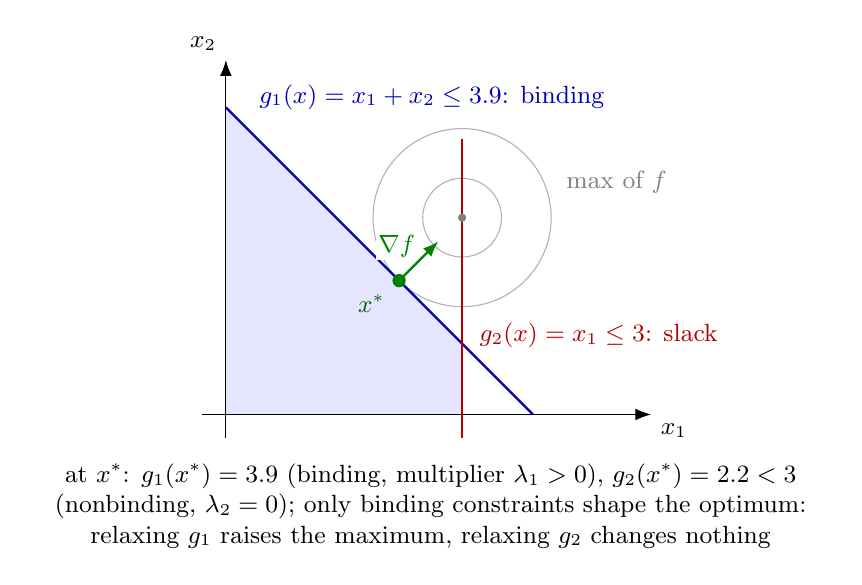
\begin{tikzpicture}[every node/.style={font=\small}, >={Latex[length=2mm]}, lab/.style={font=\small, fill=white, inner sep=1pt}]
	\fill[blue!10] (0,0) -- (3,0) -- (3,0.9) -- (0,3.9) -- cycle;
	\foreach \r in {0.5,1.131} {\draw[gray!60] (3,2.5) circle (\r);}
	\draw[->] (-0.3,0) -- (5.4,0) node[below right] {$x_1$};
	\draw[->] (0,-0.3) -- (0,4.5) node[above left] {$x_2$};
	\draw[blue!70!black, thick] (3.9,0) -- (0,3.9);
	\node[blue!70!black, anchor=south west, font=\small] at (0.3,3.75) {$g_1(x)=x_1+x_2\le3.9$: binding};
	\draw[red!70!black, thick] (3,-0.3) -- (3,3.5);
	\node[red!70!black, anchor=west, font=\small] at (3.1,1.0) {$g_2(x)=x_1\le3$: slack};
	\fill[gray] (3,2.5) circle (1.5pt);
	\node[gray, font=\small, anchor=west] at (4.2,2.95) {max of $f$};
	\draw[->, green!50!black, thick] (2.2,1.7) -- (2.7,2.2) node[midway, above left, lab] {$\nabla f$};
	\fill[green!50!black] (2.2,1.7) circle (2.4pt);
	\node[green!40!black, anchor=north east, font=\small] at (2.14,1.65) {$x^\ast$};
	\node[anchor=north, align=flush center, text width=10cm] at (2.6,-0.5) {at $x^\ast$: $g_1(x^\ast)=3.9$ (binding, multiplier $\lambda_1>0$), $g_2(x^\ast)=2.2<3$ (nonbinding, $\lambda_2=0$); only binding constraints shape the optimum: relaxing $g_1$ raises the maximum, relaxing $g_2$ changes nothing};
\end{tikzpicture}
\end{document}
